% !TeX program = pdfLaTeX
\documentclass[12pt]{article}
\usepackage{amsmath}
\usepackage{graphicx,psfrag,epsf}
\usepackage{enumerate}
\usepackage{natbib}
\usepackage{textcomp}
\usepackage[hyphens]{url} % not crucial - just used below for the URL
\usepackage{hyperref}
\providecommand{\tightlist}{%
  \setlength{\itemsep}{0pt}\setlength{\parskip}{0pt}}

%\pdfminorversion=4
% NOTE: To produce blinded version, replace "0" with "1" below.
\newcommand{\blind}{0}

% DON'T change margins - should be 1 inch all around.
\addtolength{\oddsidemargin}{-.5in}%
\addtolength{\evensidemargin}{-.5in}%
\addtolength{\textwidth}{1in}%
\addtolength{\textheight}{1.3in}%
\addtolength{\topmargin}{-.8in}%

%% load any required packages here



% Pandoc citation processing


\begin{document}


\def\spacingset#1{\renewcommand{\baselinestretch}%
{#1}\small\normalsize} \spacingset{1}


%%%%%%%%%%%%%%%%%%%%%%%%%%%%%%%%%%%%%%%%%%%%%%%%%%%%%%%%%%%%%%%%%%%%%%%%%%%%%%

\if0\blind
{
  \title{\bf An Examination of Sport Climbing Competition Format and
Scoring System}

  \author{
        Quang Nguyen \\
    LUC\\
     and \\     Hannah Butler \\
    CSU\\
     and \\     Gregory Matthews \\
    LUC\\
      }
  \maketitle
} \fi

\if1\blind
{
  \bigskip
  \bigskip
  \bigskip
  \begin{center}
    {\LARGE\bf An Examination of Sport Climbing Competition Format and
Scoring System}
  \end{center}
  \medskip
} \fi

\bigskip
\begin{abstract}
The purpose of this paper is to investigate sport climbing, one of the
sports making its debut on the Olympics stage at Tokyo 2020. In
particular, we take a closer look at the controversial competition
format and scoring system of sport climbing\ldots{} Simulation. Data
Analysis: drop and re-rank, correlations
\end{abstract}

\noindent%
{\it Keywords:} sport climbing, scoring system, 2020 Summer Olympics
\vfill

\newpage
\spacingset{1.45} % DON'T change the spacing!

\hypertarget{introduction}{%
\section{Introduction}\label{introduction}}

In 2016, the International Olympic Committee announced the addition of
five new sports to the 2020 Summer Olympics in Tokyo, Japan, which would
then reschedule for 2021 due to the impact of the COVID-19 global
pandemic. The five new features to Tokyo 2020's competitions program
include baseball/softball, karate, skateboard, sports climbing, and
surfing. One of the new sports, sport climbing, got our attention,
specifically because of its unique scoring system and the fact that only
one set of medals is awarded for each gender.

Sport climbing at the 2020 Tokyo Olympics consists of three disciplines:
speed climbing, bouldering, and lead climbing. Speed climbing takes
place on a standardized course and competitors try to reach the top of
the course as fast as possible. For Tokyo 2020, speed climbing is being
contested in a head-to-head format with ranks determined by how far a
competitor advances in the bracket. In bouldering, contestants have a
fixed amount of time to complete as many courses as they can. Winners
are determined based on who completes the most courses and ties are
broken based on who had the fewest attempts. Ties are further broken by
the competitor achieved the most ``zone holds'', which are holds
approximately halfway through each course. Finally, in lead climbing, an
athlete gets one point for each hold that they reach, so whoever reaches
the highest point on the wall is the winner. Each lead climber only gets
one attempt and when they fall their attempt is over. These three
different climbing disciplines demand different sets of skills and,
often, athletes specialize in a single event. However, since only one
set of Olympic medals is awarded to sport climbing, rather than choosing
only one of these disciplines to include in the Olympics, all three
events were chosen to be included as a sort of climbing triathlon.

At the 2020 Summer Olympics, both men's and women's sport climbing
competitions begin with 20 climbers who has previously qualified for the
Olympics from qualifying events held in 2019 and 2020. All 20 athletes
compete in each of the three disciplines in the qualification round, and
their performances in each concentration are ranked from 1 to 20. A
competitor's total score is then computed as the product of their ranks
in the three events and the lower product is better; specifically,
\begin{equation}
Score_i = R^S_i\times R^B_i\times R^L_i,
\end{equation} where \(R^S_i\), \(R^B_i\), and \(R^L_i\) are the ranks
of the \(i\)-th competitor in speed climbing, bouldering, and lead
climbing, respectively.

The top 8 finishers in the qualification round advance to the finals
where they once again compete in all three of speed climbing,
bouldering, and lead climbing. The total score for each climber in the
final stage is determined by multiplying their ranks in each discipline,
similar to the qualification round. This implies that the climber with
the lowest product of ranks in the final wins the gold medal. This type
of scoring system heavily rewards high finishes and relatively ignores
poor finishes. For instance, if climber A finished 1st, 20th, and 20th
and climber B finished 10th, 10th, and 10th, climber B would have a
score of 1000 whereas climber A would have a much better score of 400,
despite finishing last in 2 out of 3 of the events.

Heavily criticized

Other sports scoring methods

The manuscript is outlined as follows. We first begin with some
descriptions of the data and methods in Section 2. Our analyses and
results are then presented in Sections 3 and 4. Finally, in Section 5,
we summarize up our main findings and provide a discussion to close out
the paper.

\hypertarget{data-and-methods}{%
\section{Data and Methods}\label{data-and-methods}}

Our first sets of data come from a simulation study that we conducted,
with the purpose of examining the rankings and scoring for climbers in
both qualification and final rounds. For each round, we performed 10000
simulations, and this was accomplished by randomly assigning the ranks
of each event to every participant, with the assumption that the ranks
are uniformly distributed. After the completion of the simulations, we
calculated the total scores for every simulated round, as well as the
final standings for the climbing athletes. The simulation results allow
to answer questions about various topics, including the distributions of
scores for qualifying and final rounds, and the probabilities of
advancing to the finals or winning a medal, given certain conditions.

Table 1 and Figure 1 are numerical and visual summaries of climbing
total score obtained from our simulated data for the qualification and
final rounds.

\begin{table}[ht]
\centering
\caption{Descriptive statistics of simulated scores for qualification and final rounds} 
\begin{tabular}{lrrrrrrrr}
  \hline
round & min & Q1 & median & Q3 & max & mean & sd & n \\ 
  \hline
Qualification & 1.00 & 240.00 & 684.00 & 1638.00 & 8000.00 & 1158.84 & 1273.48 & 200000 \\ 
  Final & 1.00 & 24.00 & 60.00 & 126.00 & 512.00 & 91.12 & 91.35 & 80000 \\ 
   \hline
\end{tabular}
\end{table}

\begin{figure}
\centering
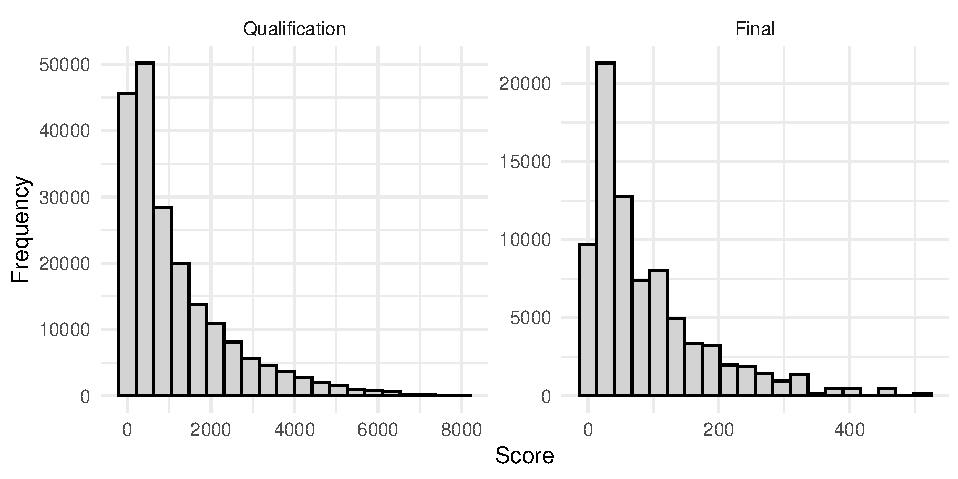
\includegraphics{draft_files/figure-latex/unnamed-chunk-5-1.pdf}
\caption{Histogram of simulated scores for qualification and final
rounds}
\end{figure}

Additionally, we rely historical results from major climbing
competitions in recent years. We collected data on climbing contests
that took place between 2018 and 2020, where the combined format was
used to determine the scores and ranks of climbers. The events include
the 2020 Continental Championships of Europe, Africa, Oceania,
Pan-America; 2019 and 2018 World Championships; 2018 Asian Games; and
2018 Youth Olympics. Data were obtained from various sources, including
the event websites, Wikipedia, and the International Federation of Sport
Climbing (IFSC). The main attributes of our datasets are the name and
nationality of the climbers; bib number (for some competitions); the
finishing place of climbers in speed climbing, bouldering, and lead
climbing; the total score (which equals the product of event ranks); and
the final rank. We utilize this data to compute the correlations between
the event ranks and final table position, as well as to look at how
often the final orderings change if one athlete is dropped and the ranks
for each discipline are re-computed.

\hypertarget{simulations}{%
\section{Simulations}\label{simulations}}

\hypertarget{uniform-ranks}{%
\subsection{Uniform Ranks}\label{uniform-ranks}}

In this section, we discuss the results of our simulations described in
Section \ref{data-and-methods}. For the qualification round, our
simulation study shows that a climber is almost guaranteed to make the
final round if they win the first event (with a 99.51\% chance of
advancing) or if they win at least one of the three climbing
concentrations (99.48\%). On the other hand, finishing last in the first
event or in any event would certainly hurt an athlete's chance of
finishing in the top 8, as the probabilities of a climber advancing
given they finish last in the first and in any event are 0.1830 and
0.1885, respectively. In addition, the average score for qualification
positions 1 to 8 are displayed in Table 2. We notice that on average,
the minimum score that one should aim for in order to move on to the
final round is about 434 (for 8th rank).

\begin{table}[ht]
\centering
\caption{The average scores for the top 10 qualification ranks according to our simulations. A climber will secure a finalist spot if they finish in the top 8.} 
\begin{tabular}{rr}
  \hline
Rank & Average score \\ 
  \hline
  1 & 36.02 \\ 
    2 & 73.61 \\ 
    3 & 115.40 \\ 
    4 & 162.23 \\ 
    5 & 216.00 \\ 
    6 & 278.16 \\ 
    7 & 350.33 \\ 
    8 & 434.59 \\ 
    9 & 532.14 \\ 
   10 & 642.33 \\ 
   \hline
\end{tabular}
\end{table}

Regarding the finals, a climber is very likely to finish in the top 3
and hence earn a medal if they win the first event (83.03\% chance) or
any event (85.01\% chance). Furthermore, according to our final
simulations, in order to obtain a climbing medal, the average scores
(rounded down) that put an athlete in position to receive gold, silver,
and bronze medals are 9, 20, and 33, respectively (see Table 3).

\begin{table}[ht]
\centering
\caption{The average scores for all final ranks according to our simulations. Ranks 1, 2, and 3 are table positions that guarantee medalist status for climbers.} 
\begin{tabular}{rr}
  \hline
Rank & Average score \\ 
  \hline
  1 & 9.67 \\ 
    2 & 20.41 \\ 
    3 & 33.26 \\ 
    4 & 50.59 \\ 
    5 & 74.76 \\ 
    6 & 110.05 \\ 
    7 & 164.43 \\ 
    8 & 265.78 \\ 
   \hline
\end{tabular}
\end{table}

\hypertarget{leave-one-climber-out}{%
\subsection{Leave-one-climber-out}\label{leave-one-climber-out}}

We would expect that if a climber with a high combined ranking is
removed from the list of competitors, the placement of lower-ranked
climbers will shift. In the most trivial case, if we were to remove the
3rd place climber, we would see 4th place climber shift to 3rd, 5th
place climber shift to 4th, etc. It is maybe less trivial that when a
climber is removed from the list, the placement of their higher-ranking
competitors may also shift. In other words, there is a non-zero
probability of seeing a change in the placement - particularly of
medalists - regardless of the fact that no changes occurred in the
performance of the remaining climbers. Real examples are given in
section 4.2. In this section, we conduct simulations to analyze the
probability of seeing a reordering of medalists when one non-medalist is
removed from the list of finalists.

\hypertarget{data-analysis}{%
\section{Data Analysis}\label{data-analysis}}

\hypertarget{rank-correlation}{%
\subsection{Rank Correlation}\label{rank-correlation}}

For our analysis on the relationship between the rankings of the events
and the final result, we used data from the 2018 Youth Olympics Women's
Qualification. Figure 2 is a scatterplot and correlation matrix between
the ranks of the individual events and the final standings, with
Kendall's Tau (Kendall Rank Correlation Coefficient) as our measure of
ordinal association between the quantities. It is evidently clear that
there exists a strong and positive correlation between the ranks of
bouldering and lead climbing, and as a results, the standings of these
two events are highly correlated with the final rankings. On the other
hand, the correlation with the final rank is not as strong for speed
climbing. Thus, speed climbers are facing a huge disadvantage in this
scoring system, compared to those that are specialized in the other two
concentrations.

\begin{figure}
\centering
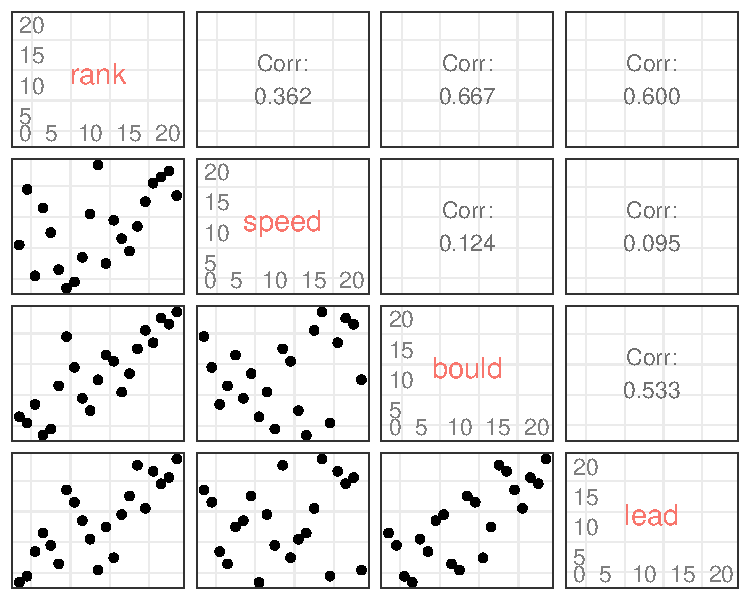
\includegraphics{draft_files/figure-latex/unnamed-chunk-9-1.pdf}
\caption{Kendall's rank correlations - 2018 World Championship, Women's
Qualification}
\end{figure}

\hypertarget{leave-one-climber-out-analysis}{%
\subsection{Leave-one-climber-out
Analysis}\label{leave-one-climber-out-analysis}}

Another interesting question that we are interested in investigating is
``What would happen to the rankings if a single climber is removed?''.

This illustrates the idea of IIA

We once again make use of data from the 2018 Youth Olympics for this
analysis, but this time we examine the final round of both men's and
women's competitions.

Figure 3 shows the plots

A single climber excluded changes things drastically, especially order
of medalists.

The cases where someone behind you drops out and your ranking changes.
Figure

\begin{figure}
\centering
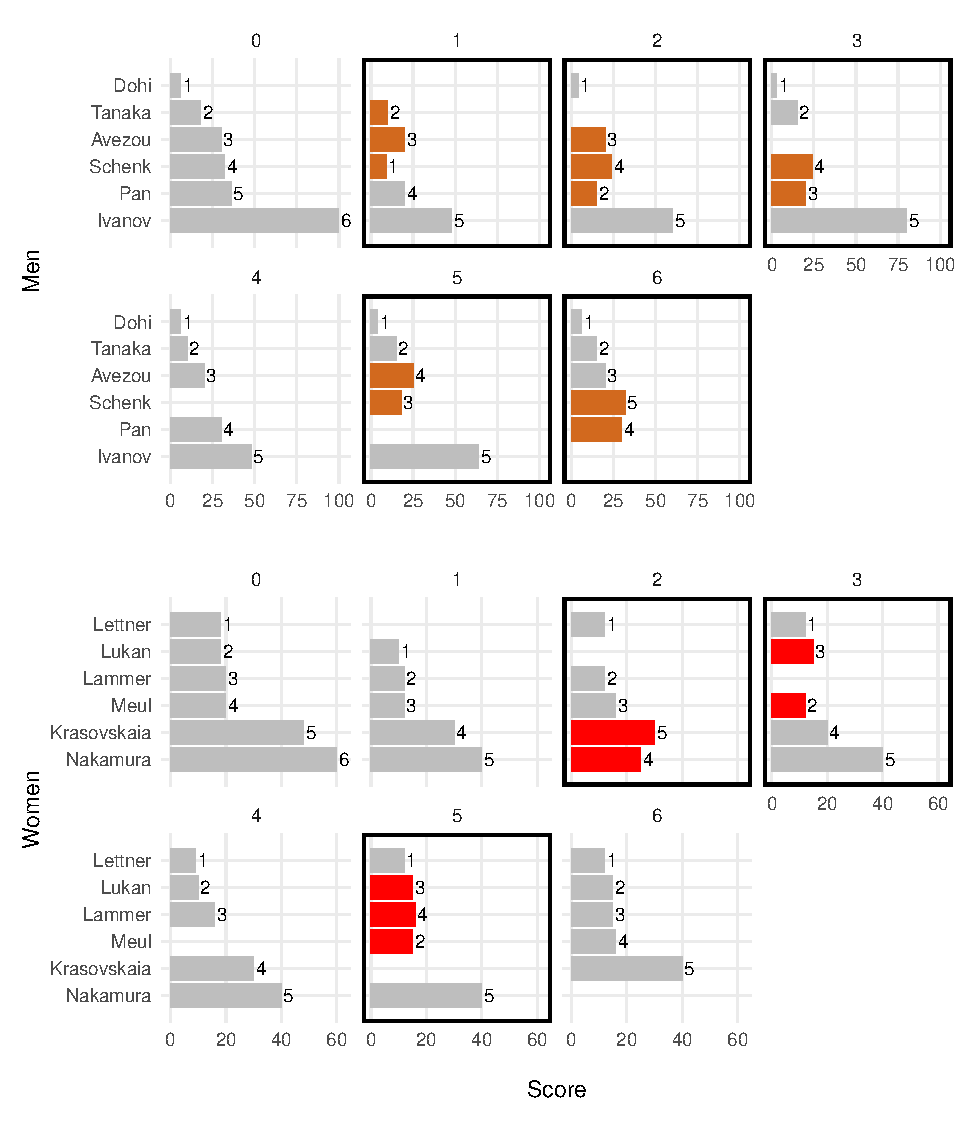
\includegraphics{draft_files/figure-latex/unnamed-chunk-12-1.pdf}
\caption{This figure illustrates the changes to the final rankings of
the 2018 Youth Olympics Men's and Women's Finals when we leave out one
climber. For each gender competition, each panel represents the rank of
the drop-out athlete, with 0 being the original final results. Each case
with a change in rank orderings is highlighted by a black panel border,
and any player with a rank change is represented by a red-filled bar}
\end{figure}

\bibliographystyle{agsm}
\bibliography{}

\end{document}
